\documentclass[11pt,oneside,a4paper]{article}

\usepackage{cite}
\usepackage{amsmath}
\usepackage{amsthm}
\usepackage{epsfig}
\usepackage{graphicx}
\usepackage{caption}
\usepackage{refstyle}
\usepackage{float}
\usepackage{array}
\usepackage{amssymb}
\usepackage{subcaption}
\usepackage{wrapfig}
\usepackage{multirow}
\usepackage{pseudocode}
\usepackage{fancybox}
\usepackage{tabularx}
\usepackage{multirow}
\usepackage{algpseudocode}
\usepackage{algorithmicx}
\usepackage{algorithm}

\usepackage[normalem]{ulem}
\usepackage{soul}
%\DeclareMathOperator*{\argmax}{arg\,max}
\DeclareMathOperator*{\argminA}{arg\,min}
%\title{ELEG636: Introduction to Machine Learning Homework \#1}
\begin{document}
%\maketitle
\title{Modern Machine Learning\\Computer Assignment \#5}
\date{\vspace{-5ex}}
\maketitle
%We thank the editor for his/her comments on the manuscript. %His/her suggestions/recommendations have significantly improved %the manuscript.
%In the following, we address each of the editor's comments in the %order in which they were mentioned.
%\\
\begin{enumerate}
	
  \item \textit{Model selection for Polynomial Regression:} implement the gradient descent algorithm for polynomial regression and choose the model with the lowest error.
  \\
  \\
  \textbf{Background:} The gradient descent algorithm for linear regression consists of updates of the form
  
  \begin{equation}\nonumber
  \begin{aligned}
  \beta_1^{k+1}=\beta_1^{k}-\alpha\sum_{i=1}^{p}\left(h_{\beta^k}(\textbf{z}_i)-y_i\right)z_{i1}\\
  \beta_2^{k+1}=\beta_2^{k}-\alpha\sum_{i=1}^{p}\left(h_{\beta^k}(\textbf{z}_i)-y_i\right)z_{i2}\\
  \vdots\\
  \beta_p^{k+1}=\beta_p^{k}-\alpha\sum_{i=1}^{p}\left(h_{\beta^k}(\textbf{z}_i)-y_i\right)z_{ip},
  \end{aligned}
  \end{equation}  
  until convergence is achieved, where $h_{\beta^k}(\textbf{z}_i)=\beta_0^k+\beta_1^k z_{i1}+\beta_2^k z_{i2}+\dots+\beta_p^k z_{ip}$.  You can assume that the algorithm has converged when the entries $\beta_j$ vary less than a specified value $\epsilon$.
  
  \textbf{Note:} Polynomial regression can be achieved by applying a transformation to the inputs $\textbf{x}$. In this particular case, the output can be expressed as $\textbf{y}=
  \beta_0+\beta_1\textbf{x}+\beta_2\textbf{x}^2+\dots+\beta_p\textbf{x}^p$, where the power operations are performed \textbf{pointwise}. Therefore the observation matrix is defined as $\textbf{X}=[\textbf{x},\textbf{x}^2,\dots, \textbf{x}^p]$
  \\
  \\
  Recall that model selection is performed by plotting the curves $J_{val}$ vs $p$, and $J_{test}$ vs $p$. Then we select the appropriate model based on the regions shown in Fig. 1.
    \begin{figure}\centering
  	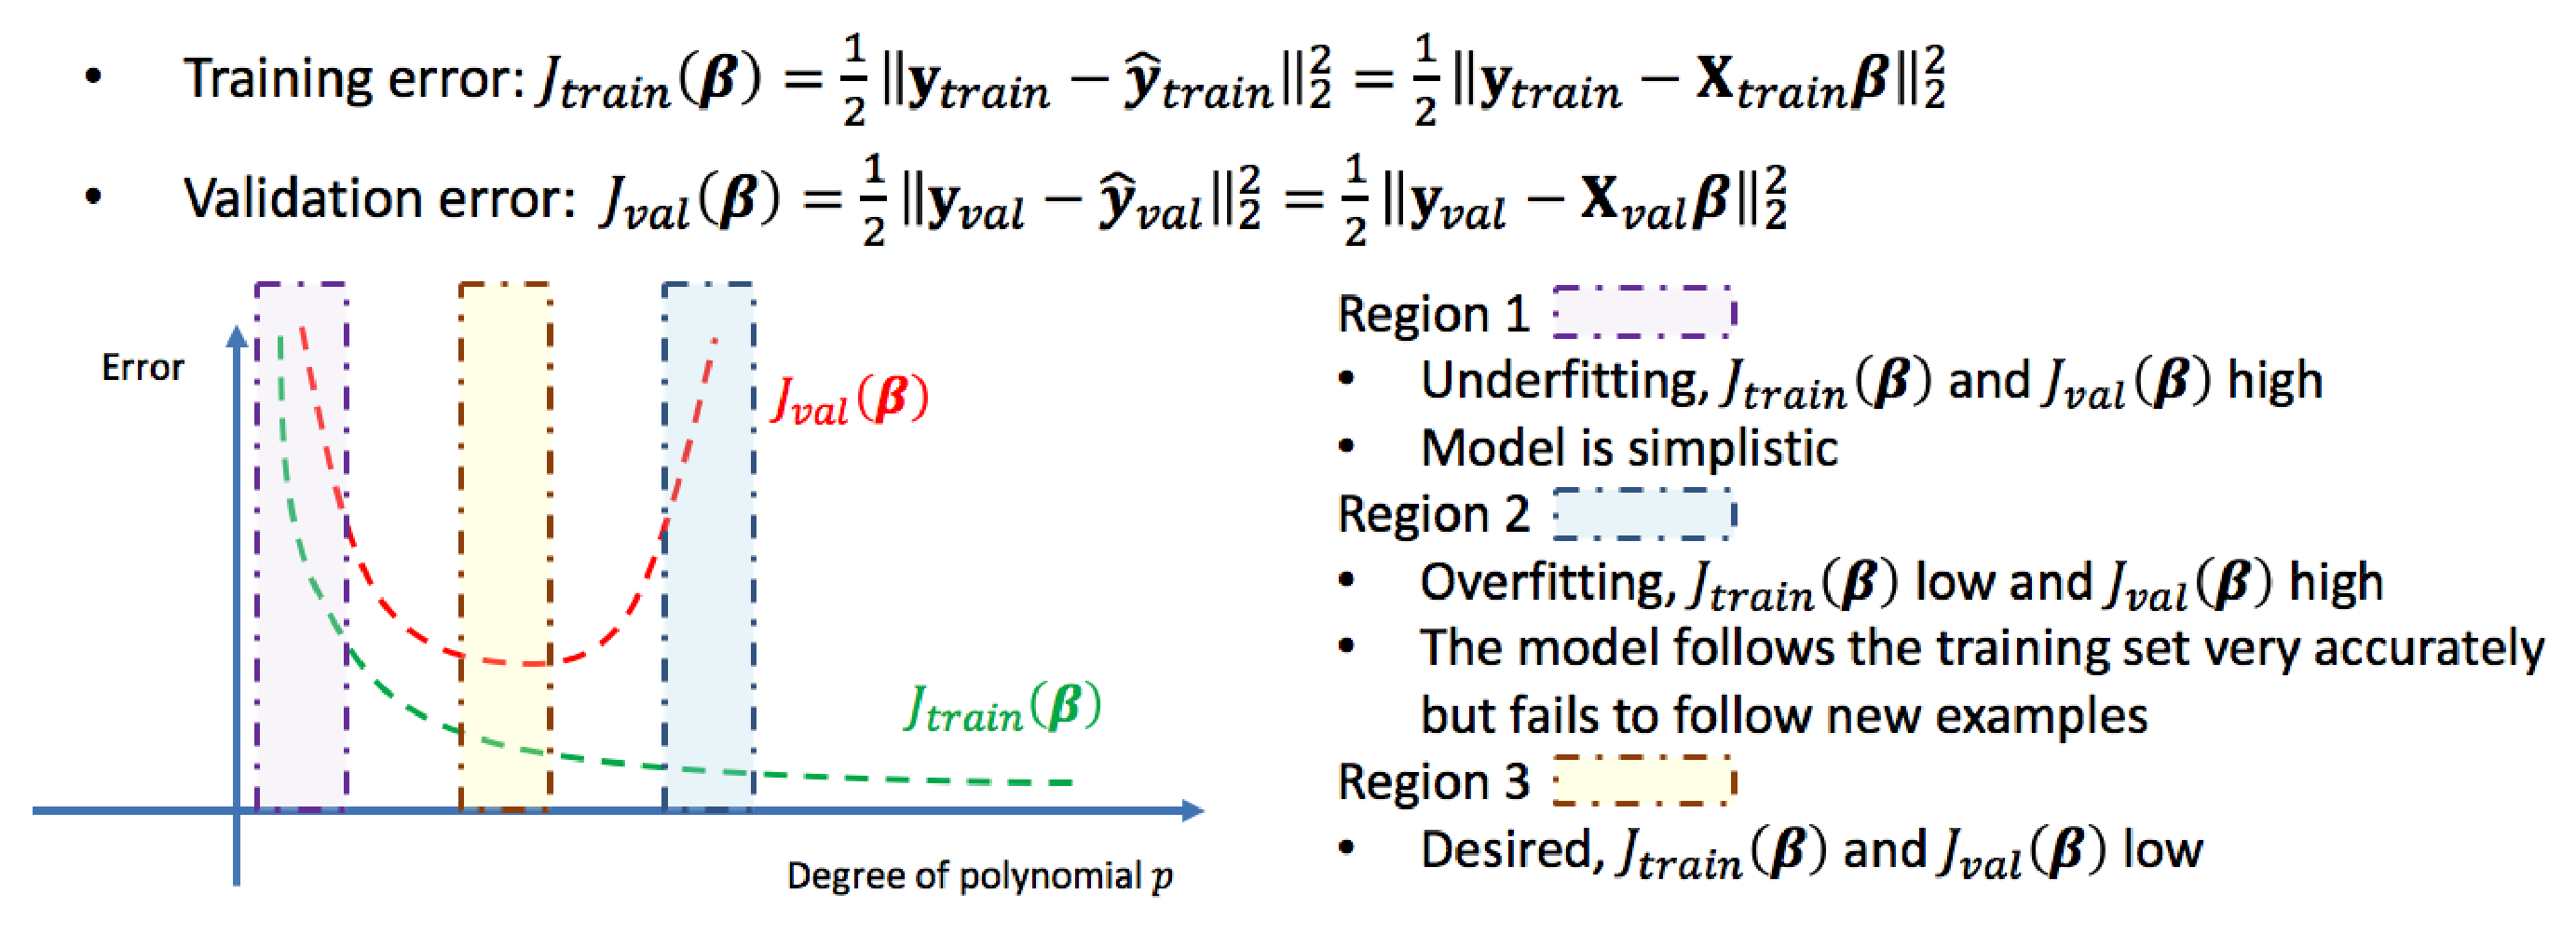
\includegraphics[height=0.4\textwidth]{model_sel.eps}
  	\caption{Model selection procedure}
  	\label{fig:MINSTimages}
  \end{figure}
  
  \pagebreak
  
  \textbf{Python files:} The script `polynomial\_regression\_example.py' uses the gradient descent to obtain the least squares solution to the transformations of the observations (also called polynomial regression). 
  The script also plots the solution obtained and the training/validation/testing erros.
  \\
  \textbf{Submission guidelines:} Your submission should include:
  \begin{itemize}
  	\item A unique \textbf{zip folder}, which should include a modified version of `polynomial\_regression\_example.py'.  You are required to learn different polynomial models with different degrees from 1 to 7, calculate the training error and validation error, and visualize the relation between the degree of polynomial and the training/validation errors like Figure 1.
	
   \item Please rename the modified file `polynomial\_regression\_example.py' replacing the word 'example' in the provided script with your last name. \textbf{This should be the main function}.
  	\item A pdf file containing a figure with the curves $J_{val}$ vs $p$, and $J_{train}$ vs $p$, for $p=1,2,3,4,5,6,7$. What order $p$ would you select for the polynomial regression and why?
  \end{itemize}

\pagebreak
  \textbf{MATLAB files:} The script eval\_learning\_alg\_example.m uses the MATLAB function $polyfit(\cdot)$ to obtain the least squares solution using feature transformations on the observations (also called polynomial regression). The script also plots the solution obtained.
  \\
  \textbf{Submission guidelines:} Your submission should include:
  \begin{itemize}
  	\item A unique \textbf{zip folder}, which should include a modified version of eval\_learning\_alg\_example.m and mypolreg.m. The structure of the function mypolreg.m is the following: $[\hat{\pmb{\beta}}, J]=\text{mypolreg}(\textbf{X},\textbf{y},p)$, where $\textbf{X}$ are the observations, $\textbf{y}$ is the output of the model $\textbf{y}= \textbf{X} \pmb{\beta}+ \pmb{\epsilon}$, where $\pmb{\epsilon}$ is Gaussian noise, and $p$ is the order of the polynomial fit. The output $\hat{\pmb{\beta}}$ contains the polynomial regression coefficients. This function should implement gradient descent to obtain the least squares solution to polynomial regression. Please insert this function where indicated in the script. Make sure the results you obtain are very close to the ones returned by the function polyfit.
  	Please rename the modified file eval\_learning\_alg\_example.m replacing the word 'example' in the provided script with your last name. For example, eval\_learning\_alg\_smith.m. \textbf{This should be the main function}.
  	\item A pdf file containing a figure with the curves $J_{val}$ vs $p$, and $J_{train}$ vs $p$, for $p=1,2,3,4,5,6,7$. What order $p$ would you select for the polynomial regression and why?
  \end{itemize} 
\end{enumerate}
%\bibliographystyle{plain}
%\bibliography{refs}

\end{document}
